\begin{figure}
    \begin{center}
        \begin{subfigure}{0.4\textwidth}
            \begin{center}
                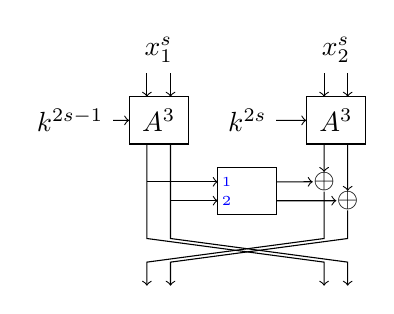
\begin{tikzpicture}[yscale=0.6, xscale=0.75]
                    % input
                    \draw (-1.5, +5.0) node(x0){$x^s_1$} ;
                    \draw (+1.5, +5.0) node(x1){$x^s_2$} ;
                    \draw[->] (-1.7, +4.5) -- (-1.7, +4.0) ;
                    \draw[->] (-1.3, +4.5) -- (-1.3, +4.0) ;
                    \draw[->] (+1.7, +4.5) -- (+1.7, +4.0) ;
                    \draw[->] (+1.3, +4.5) -- (+1.3, +4.0) ;
                    % S-Box layer
                    \draw (-3.0, +3.5) node(k0){$k^{2s-1}$} ;
                    \draw (+0.0, +3.5) node(k1){$k^{2s}$} ;
                    \draw[->] (k0) -- (-2.0, +3.5) ;
                    \draw[->] (k1) -- (+1.0, +3.5) ;
                    \draw (-2.0, +3.0) rectangle node[pos=0.5]{$A^3$} (-1.0, +4.0) ;
                    \draw (+1.0, +3.0) rectangle node[pos=0.5]{$A^3$} (+2.0, +4.0) ;
                    % Linear layer
                    \draw (-0.5, +1.5) rectangle node[pos=0.5]{$\Lthirty$} (+0.5, +2.5) ;
                    \draw (-0.35, +2.2) node{\color{blue} \tiny 1} ;
                    \draw (-0.35, +1.8) node{\color{blue} \tiny 2} ;
                    \draw (+1.3, +2.2) node[inner sep=0](xor0){$\oplus$} ;
                    \draw (+1.7, +1.8) node[inner sep=0](xor1){$\oplus$} ;
                    \draw[->] (-1.7, 3.0) -- (-1.7, 1.0) -- (+1.3, 0.5) -- (+1.3, 0.0) ;
                    \draw[->] (-1.3, 3.0) -- (-1.3, 1.0) -- (+1.7, 0.5) -- (+1.7, 0.0) ;
                    \draw[->] (+1.3, 3.0) -- (xor0) ;
                    \draw[->] (+1.7, 3.0) -- (xor1) ;
                    \draw[->] (+0.5, 2.2) -- (xor0) ;
                    \draw[->] (+0.5, 1.8) -- (xor1) ;
                    \draw[->] (xor0) -- (+1.3, 1.0) -- (-1.7, 0.5) -- (-1.7, 0.0) ;
                    \draw[->] (xor1) -- (+1.7, 1.0) -- (-1.3, 0.5) -- (-1.3, 0.0) ;
                    \draw[->] (-1.7, 2.2) -- (-0.5, 2.2) ;
                    \draw[->] (-1.3, 1.8) -- (-0.5, 1.8) ;
                \end{tikzpicture}
                \caption{\label{fig:sparx-64-round}Step structure.}
            \end{center}
        \end{subfigure}
        \hspace{1em}
        \begin{subfigure}{0.23\textwidth}
            \begin{center}
                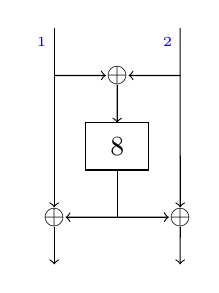
\begin{tikzpicture}[yscale=0.6, xscale=0.8]
                    \draw (+1.0, 5.0) node[inner sep=0](xorT){$\oplus$};
                    \draw[->] (+0.0, 5.0) -- (xorT) ;
                    \draw[->] (+2.0, 5.0) -- (xorT) ;
                    \draw (+0.0, 2.0) node[inner sep=0](xorL){$\oplus$};
                    \draw (+2.0, 2.0) node[inner sep=0](xorR){$\oplus$};
                    \draw[->] (+0.0, 6.0) -- (xorL) ;
                    \draw[->] (xorL) -- (+0.0, 1.0);
                    \draw[->] (+2.0, 6.0) -- (xorR) ;
                    \draw[->] (xorR) -- (+2.0, 1.0);
                    \draw (+0.5, +3.0) rectangle node[pos=0.5]{$\lll 8$} (+1.5, 4.0) ;
                    \draw[->] (xorT) -- (+1.0, +4.0) ;
                    \draw (+1.0, +3.0) -- (+1.0, +2.0) ;
                    \draw[->] (+1.0, +2.0) -- (xorL) ;
                    \draw[->] (+1.0, +2.0) -- (xorR) ;
                    \draw (-0.2, +5.7) node{\color{blue} \tiny 1} ;
                    \draw (+1.8, +5.7) node{\color{blue} \tiny 2} ;
                \end{tikzpicture}
                \caption{\label{fig:sparx-64-L}$\Lthirty$.}
            \end{center}
        \end{subfigure}
    \end{center}
    \FigDef{sparx64}{An overview of \spnARXinstance{64}{128}. Branches are 16-bit (except for the keys).}
\end{figure}
 